\documentclass[aspectratio=169,11pt]{beamer}

% Shared style (ib-tutorials.sty at the repo root).
\makeatletter\def\input@path{{./}{../}}\makeatother
\usepackage{ib-tutorials}

\usepackage[utf8]{inputenc}
\usepackage{amsmath,amssymb}
\usepackage{booktabs}
\usepackage{array}
\newcolumntype{L}[1]{>{\raggedright\arraybackslash}p{#1}}
\usepackage{graphicx}
\graphicspath{{../pictures/3-ibamr-fundamentals/}{pictures/3-ibamr-fundamentals/}}
\usepackage{xcolor}
\usepackage{listings}
\usepackage{tikz}
\usetikzlibrary{arrows.meta,positioning,shapes.geometric,fit,calc}
\usepackage{hyperref}

\newcommand{\sourcecredit}[1]{\vfill\hfill{\tiny\textcolor{DarkGray}{#1}}}

\lstset{
  basicstyle=\ttfamily\scriptsize\color{BlackGray},
  keywordstyle=\color{NavyBlue}\bfseries,
  commentstyle=\color{DarkGray}\itshape,
  stringstyle=\color{OliveGreen},
  showstringspaces=false,
  columns=fullflexible,
  keepspaces=true,
  breaklines=true,
  breakindent=1em,
  frame=single,
  framerule=0.4pt,
  rulecolor=\color{LightGray},
  backgroundcolor=\color{LightGray!30},
  xleftmargin=0.25em,
  xrightmargin=0.25em
}
\lstdefinestyle{shell}{morecomment=[l]{\#}}
\lstdefinestyle{input}{morecomment=[l]{//}}
\lstdefinestyle{matlab}{morecomment=[l]{\%}}
\lstdefinestyle{python}{morecomment=[l]{\#}}
\lstdefinestyle{data}{}
\lstdefinestyle{tiny}{basicstyle=\ttfamily\tiny\color{BlackGray}}
\lstdefinestyle{inputtiny}{morecomment=[l]{//},basicstyle=\ttfamily\tiny\color{BlackGray}}
\lstdefinestyle{cpptiny}{language=C++,morecomment=[l]{//},basicstyle=\ttfamily\tiny\color{BlackGray}}
\lstdefinestyle{matlabtiny}{morecomment=[l]{\%},basicstyle=\ttfamily\tiny\color{BlackGray}}

\title[Non-dimensionalization]{Non-dimensionalization}
\subtitle{Reynolds, Strouhal, Womersley and P\'eclet numbers, dimensionless stiffnesses and forces, and how to match a simulation to reality}
\author[Miller]{Laura A. Miller}
\institute[UArizona]{Department of Mathematics, University of Arizona}
\date{Using IB Software \textbullet\ Part III \textbullet\ Chapter 8b}

\begin{document}

% 1
\begin{frame}[plain]
\maketutorialtitlepanel{%
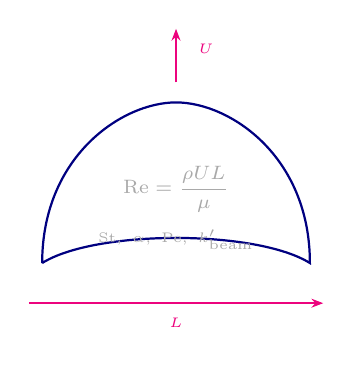
\begin{tikzpicture}[scale=0.85]
  \draw[NavyBlue,thick] (0,0) .. controls (0,1.6) and (1.2,2.4) .. (2.0,2.4) .. controls (2.8,2.4) and (4.0,1.6) .. (4.0,0) .. controls (3.2,0.5) and (0.8,0.5) .. (0,0);
  \draw[-{Stealth[length=1.5mm]},RubineRed,thick] (-0.2,-0.6) -- (4.2,-0.6);
  \node[font=\tiny,text=RubineRed] at (2.0,-0.9) {$L$};
  \draw[-{Stealth[length=1.5mm]},RubineRed,thick] (2.0,2.7) -- (2.0,3.5);
  \node[font=\tiny,text=RubineRed] at (2.45,3.2) {$U$};
  \node[font=\scriptsize,text=DarkGray] at (2.0,1.1) {$\mathrm{Re}=\dfrac{\rho U L}{\mu}$};
  \node[font=\tiny,text=DarkGray] at (2.0,0.35) {$\mathrm{St},\ \alpha,\ \mathrm{Pe},\ k'_{\mathrm{beam}}$};
\end{tikzpicture}}
\end{frame}

% 2
\begin{frame}{Learning goals}
\label{fr:goals}
\small By the end of this chapter you should be able to:
\begin{enumerate}
  \item choose a characteristic length and velocity for a model, write the Navier--Stokes equations in dimensionless form, and read a Reynolds number as a statement about the flow;
  \item define and compute the Strouhal, Womersley and P\'eclet numbers, the dimensionless force, drag and lift coefficients, and the dimensionless bending and stretching stiffnesses, in the conventions this series and the theory series share;
  \item take a real animal or organ (a jellyfish, a leaf, a glycocalyx fibre) and set up a simulation that matches its dimensionless numbers, in real units or in unit scales, and know which numbers must be matched;
  \item turn an IBAMR output (the \code{integral\{F\}} line, a tip position, a period) into a dimensionless result and report it with the scales it depends on;
  \item recognize the mistakes: an inverted Strouhal number, a 3D formula in a 2D model, matching the Reynolds number alone, and estimates mistaken for physics.
\end{enumerate}
\begin{punchbox}
\footnotesize The derivations live in the theory series' \emph{Nondimensionalization and similarity} deck (slide \ref{fr:theory}); this chapter keeps the course's statements, corrects them where needed, and applies them to the examples.
\end{punchbox}
\end{frame}

% 3
\begin{frame}{How this chapter was checked}
\label{fr:checked}
\begin{itemize}\footnotesize
  \item The definitions and formulas were compared line by line with the theory series' deck \emph{Nondimensionalization and similarity} (Module 0-2, 33 slides, 2026), which was built from the same 2015--2020 lectures; the two use the same conventions ($\mathcal{F}' = \mathcal{F}/(\rho U^2 L)$, $k'_{\mathrm{beam}} = k_{\mathrm{beam}}/(\rho U^2L^3)$ in 2D, $\mathrm{St}_L = fL/U$), and chapter 8a's estimates use them too.
  \item Every number about an example is computed from its input file, generator or README on the \code{master-tutorial} branch; the drag coefficient of the leaf is computed from the \code{integral\{F\}} lines of the shipped run with a script that is in the references.
  \item The third-party material of the old slides (Wikipedia screenshots of definitions, tables and plots) is replaced by retyped tables and own drawings, with the sources named on each slide.
  \item The contradictions between the 2014, 2015, 2017, 2018 and 2020 versions (the Strouhal definition, the $L^3$ versus $L^4$ beam number, the ``little bending'' threshold of $1$, $1$--$10$ or $10$) are resolved on slides \ref{fr:strouhal}, \ref{fr:kbeam} and \ref{fr:changed}.
\end{itemize}
\vspace{1mm}
\begin{punchbox}
\small Slide numbers refer to this deck; chapter numbers (5, 6, 7, 8a, 9a, 10, 11, 16, 26) to the other chapters of this series.
\end{punchbox}
\end{frame}

% 4
\begin{frame}{Where the derivations are: the theory series}
\label{fr:theory}
\small \emph{Fluid Dynamics and IBM Theory}, Module 0-2, \emph{Nondimensionalization and similarity} (33 slides): \url{https://github.com/fairyflies9/Fluid-Dynamics-and-IBM-Theory/blob/main/0-Intro-to-Fluid-Mechanics/0-2-Nondimensionalization.pdf}
\vspace{1mm}

\scriptsize
\begin{tabular}{@{}L{0.44\textwidth}L{0.46\textwidth}@{}}
\toprule
Theory deck frames & What this chapter adds\\
\midrule
Why nondimensionalize; characteristic scales; dimensionless variables and derivatives; the inertial form of Navier--Stokes; the viscous normalization & the two ways to set up an IBAMR run (real units or unit scales) and the examples' choices of $U$ and $L$\\
Reynolds, Strouhal (two definitions), Womersley (with the canine table and a worked check), P\'eclet & the regimes drawn, the biological ranges, and each number computed for the examples\\
Force scales for a 2D model; bending and stretching coefficients; viscosity and Reynolds-number matching & drag and lift coefficients from \code{integral\{F\}}, with the leaf's $C_D(t)$ measured\\
Flexural rigidity; Young's modulus; second moment of area; converting structural parameters; the beam, load and spring starting estimates; damping & how IBAMR's spring force defines $K$ (the energy, the tension, the code), the IB equations with their units, and the growing-springs worked example\\
Efficiency; cost of transport; the checklist & matching more than Re, three worked conversions (jellyfish, leaf, glycocalyx), reporting dimensionless results, what can go wrong\\
\bottomrule
\end{tabular}

\vspace{2mm}
\small Read the theory deck for \emph{why}; read this one for \emph{how, in IBAMR}. Both are built from the same lectures, so nothing is lost by the split.
\end{frame}

% 5
\begin{frame}{Why non-dimensionalize?}
\label{fr:why}
\small From the 2015, 2018 and 2020 lectures:
\begin{itemize}
  \item ``You either need to work in real units (real size of a jellyfish, insect, etc.) or you need to report dimensionless values.''
  \item ``It allows you to easily do parameter sweeps while changing only one variable.''
  \item ``In a research paper, you either need to work in real units or you need to report dimensionless values.''
  \item ``The challenge with dimensionless simulations is that you must match all length/time/velocity scales.''
  \item ``In the outline that follows, $U'$ will denote dimensionless $U$, and so on.''
\end{itemize}
\vspace{1mm}
\begin{punchbox}
\small A simulation is one point in parameter space. Dimensionless numbers say which other points it stands for: every leaf, stream and fluid with the same $\mathrm{Re}$ and the same $k'_{\mathrm{beam}}$ bends the same way, whatever the metres and seconds. That is \al{dynamic similarity}, and it is why one run of IB/03 can be compared with a leaf in a flume or a flag in the wind, once both are reduced to the same numbers.
\end{punchbox}
\vspace{1mm}
\small Chapter 8a changed parameters one at a time; this chapter says which combinations of them matter.
\end{frame}

% 6
\begin{frame}{Two ways to set up a run: real units, or unit scales}
\label{fr:twoways}
\small From the 2014 ``What can go wrong'' lecture: ``Sometimes it's easiest to construct geometries and velocities around unity. If you just match them to reality, you don't have to worry about matching every important quantity. If you have a lot of results that are not matched to reality, then you have to make things dimensionless and compare them to the real thing.''
\vspace{1mm}

\scriptsize
\begin{tabular}{@{}L{0.14\textwidth}L{0.38\textwidth}L{0.38\textwidth}@{}}
\toprule
 & Real units (the IB set) & Unit scales (the IBFE set)\\
\midrule
how & SI throughout: a $1$ m box, $\rho = 1000$, a viscosity chosen for the regime, speeds in m/s, seconds & $\rho = 1$, $L = 1$ (or the body's size $= 1$), $U = 1$ or close, $\mu = 1/\mathrm{Re}$; IBFE/10 writes \code{MU = 1.0/Re}\\
advantages & every number is a physical one; nothing to convert; ``imagine what this thing would be in reality'' is immediate & the input file \emph{is} the dimensionless statement; sweeps in $\mathrm{Re}$ and $k'$ are one-line edits; results come out as coefficients\\
cost & to compare with another case, divide by the scales afterwards; the example's $\mu = 100$ is honey, not water, which surprises newcomers & the scales must be remembered when a result is turned back into metres and seconds, and every other number ($\mathrm{St}$, $k'$, $\mathrm{Pe}$) must be matched by hand\\
\bottomrule
\end{tabular}

\vspace{2mm}
\small Both are right. What is wrong is a mixture: SI stiffnesses in a $\rho = 1$ input (chapter 8a). Whichever you use, write the scales $L$, $U$, $\rho$ at the top of the input file as comments, and the dimensionless numbers under them.
\end{frame}

% 7
\begin{frame}{Table of dimensions}
\label{fr:dims}
\footnotesize Retyped from the 2018 ``Dimensions continued'' deck, with the structural constants of chapter 6 added. SI base units: kg, m, s.

\tiny
\begin{tabular}{@{}L{0.26\textwidth}L{0.14\textwidth}L{0.22\textwidth}L{0.24\textwidth}@{}}
\toprule
Measurement & Unit & Derivation & In base units\\
\midrule
frequency & hertz (Hz) & $1/\mathrm{s}$ & s$^{-1}$\\
force & newton (N) & $\mathrm{kg\,m/s^2}$ & kg m s$^{-2}$\\
pressure, stress & pascal (Pa) & $\mathrm{N/m^2}$ & kg m$^{-1}$ s$^{-2}$\\
energy, work & joule (J) & $\mathrm{N\,m}$ & kg m$^2$ s$^{-2}$\\
power & watt (W) & $\mathrm{J/s}$ & kg m$^2$ s$^{-3}$\\
dynamic viscosity $\mu$ & Pa s (poise $= 0.1$ Pa s) & $\mathrm{N\,s/m^2}$ & kg m$^{-1}$ s$^{-1}$\\
kinematic viscosity $\nu = \mu/\rho$ & m$^2$/s (stokes $= 10^{-4}$ m$^2$/s) & & m$^2$ s$^{-1}$\\
density $\rho$ & kg/m$^3$ & & kg m$^{-3}$\\
\midrule
spring stiffness $K$ (tension per unit strain) & N (3D); N/m per unit depth (2D) & chapter 6 & \\
flexural rigidity $EI$ & N m$^2$ (3D); N m per unit depth (2D) & $E$ [Pa] $\times$ $I$ [m$^4$] & \\
target stiffness $\kappa$ (per unit length) & N/m$^2$ & & \\
file values & $K/\Delta s$, $EI/\Delta s^3$, $\kappa/\Delta s$ & chapter 6 & \\
\bottomrule
\end{tabular}

\footnotesize Water: $\rho = 1000$ kg/m$^3$, $\mu = 10^{-3}$ Pa s, $\nu = 10^{-6}$ m$^2$/s. Air: $\rho = 1.2$, $\mu = 1.8\times10^{-5}$, $\nu = 1.5\times10^{-5}$. The IB examples' $\mu = 4$ to $100$ are honey to tar.
\end{frame}

% 8
\begin{frame}{Choose a characteristic length and velocity}
\label{fr:scales}
\begin{columns}[T,onlytextwidth]
\begin{column}{0.5\textwidth}
\small The 2018 text: ``Choose a characteristic velocity, $U$. This might be the free stream velocity, the velocity of the object, the maximum velocity in a pipe. Choose a characteristic length, $L$. This might be the pipe diameter, a wing chord, the length of an animal. The particular choice of characteristic scales is not as important as being consistent. In a numerical simulation, consider a domain length of $10L$ or so (depending on the application).''
\vspace{1mm}

\small The 2015/2020 version: ``It is easiest to set your jellyfish bell diameter, insect wing chord, or fin chord as the characteristic length. Then the domain will be bigger, of size $10L$ or so.''
\end{column}
\begin{column}{0.48\textwidth}
\scriptsize
\begin{tabular}{@{}L{0.22\textwidth}L{0.32\textwidth}L{0.3\textwidth}@{}}
\toprule
example & $U$ & $L$\\
\midrule
IB/03 leaf & stream, $0.1$ m/s & leaf length, $0.1$ m\\
IB/02 channel & peak inlet, $1$ m/s & channel width, $1$ m\\
IB/08 glycocalyx & shear flow at the tip, $0.0156$ m/s & fibre height, $0.156$ m\\
IB/04 cylinders & row speed, $0.2$ m/s & cylinder diameter, $5$ mm\\
IB/07 plates & plate speed, $0.2$ m/s & plate length, $0.1$ m\\
IB/01 band & its own, $\sim0.02$ m/s & diameter, $0.2$ m\\
IBFE/01 plate & tether, $0.5$ & plate length, $1$\\
IBFE/10 tank & stream, $0.1$ & plate width, $2$\\
\bottomrule
\end{tabular}

\vspace{1mm}
\small The box-to-body ratio: $10$ for IB/03 and IB/07, $5$ for IB/02, $2$ for the IBFE plates (periodic), $16$ along the stream for IBFE/10. Below about $5$ the walls or the periodic images take part (chapters 7, 16).
\end{column}
\end{columns}
\end{frame}

% 9
\begin{frame}{The Navier--Stokes equations without dimensions}
\label{fr:ns}
\small With $\mathbf{x} = L\mathbf{x}'$, $\mathbf{u} = U\mathbf{u}'$, $t = (L/U)\,t'$, $p = \rho U^2 p'$ and $\nabla = \nabla'/L$, the incompressible Navier--Stokes equations
\[
  \rho\Bigl(\frac{\partial\mathbf{u}}{\partial t} + \mathbf{u}\cdot\nabla\mathbf{u}\Bigr) = -\nabla p + \mu\nabla^2\mathbf{u} + \mathbf{F}, \qquad \nabla\cdot\mathbf{u} = 0
\]
become (the 2018 slide's own picture, retyped)
\[
  \frac{\partial\mathbf{u}'}{\partial t'} + \mathbf{u}'\cdot\nabla'\mathbf{u}' = -\nabla' p' + \frac{1}{\mathrm{Re}}\nabla'^2\mathbf{u}' + \mathbf{F}', \qquad \mathrm{Re} = \frac{\rho U L}{\mu}, \qquad \mathbf{F}' = \frac{L}{\rho U^2}\,\mathbf{F}.
\]
\begin{itemize}
  \item This is the \al{inertial} scaling: pressure measured in $\rho U^2$. It is the natural one when $\mathrm{Re} \gtrsim 1$.
  \item For $\mathrm{Re} \ll 1$ the \al{viscous} scaling, $p = (\mu U/L)\,p'$, gives $\mathrm{Re}\,(\partial_{t'}\mathbf{u}' + \mathbf{u}'\cdot\nabla'\mathbf{u}') = -\nabla'p' + \nabla'^2\mathbf{u}' + \mathbf{F}'$, and dropping the left side is Stokes flow. The two scalings describe the same equation; they differ in which term is set to size one (theory deck, ``Viscous normalization'').
  \item An IBFE input with $\rho = 1$, $U = L = 1$ and \code{MU = 1/Re} is literally the first form. An IB input in SI is the dimensional form, and $\mathrm{Re}$ is computed afterwards.
\end{itemize}
\small The Eulerian force $\mathbf{F}$ is what the structure spreads onto the grid (chapter 5); its scale is $\rho U^2/L$, a pressure gradient. Slide \ref{fr:ibunits} has the units of the whole IB system.
\end{frame}

% 10
\begin{frame}{The Reynolds number and the flow regimes}
\label{fr:re}
\begin{columns}[T,onlytextwidth]
\begin{column}{0.62\textwidth}
\footnotesize $\mathrm{Re} = \rho UL/\mu = UL/\nu$: inertial forces over viscous forces, or the ratio of the viscous time $L^2/\nu$ to the advective time $L/U$.
\begin{itemize}
  \item $\mathrm{Re} \ll 1$: creeping (Stokes) flow; symmetric fore and aft, no wake, reversible; forces $\propto \mu U L$.
  \item $\mathrm{Re} \sim 1$--$10$: a steady, slightly asymmetric flow; the comfortable band for the IB method (chapter 8a).
  \item $\mathrm{Re} \sim 50$--$200$: a pair of attached eddies, then periodic vortex shedding (a K\'arm\'an street, $\mathrm{St} \approx 0.2$).
  \item $\mathrm{Re} \sim 10^4$--$10^5$: a turbulent wake behind a laminar boundary layer; forces $\propto \rho U^2 L^2$.
  \item $\mathrm{Re} > 10^5$--$10^6$: the boundary layer itself becomes turbulent and the wake narrows (the drag crisis).
\end{itemize}
\end{column}
\begin{column}{0.36\textwidth}
\centering
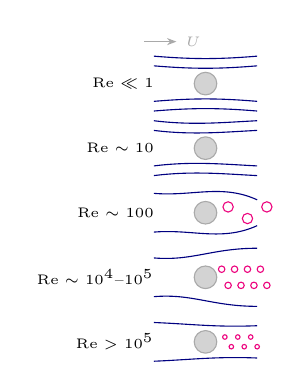
\begin{tikzpicture}[scale=0.41,every node/.style={font=\tiny}]
  \foreach \y/\lab in {8/{$\mathrm{Re} \ll 1$},6/{$\mathrm{Re} \sim 10$},4/{$\mathrm{Re} \sim 100$},2/{$\mathrm{Re} \sim 10^4$--$10^5$},0/{$\mathrm{Re} > 10^5$}}{
    \node[anchor=east] at (-0.3,\y) {\lab};
    \fill[LightGray] (1.0,\y) circle (0.35);
    \draw[DarkGray] (1.0,\y) circle (0.35);}
  % creeping: symmetric streamlines
  \foreach \d in {0.55,0.85}{\draw[NavyBlue] (-0.6,8+\d) .. controls (0.6,8+\d-0.1) and (1.4,8+\d-0.1) .. (2.6,8+\d); \draw[NavyBlue] (-0.6,8-\d) .. controls (0.6,8-\d+0.1) and (1.4,8-\d+0.1) .. (2.6,8-\d);}
  % Re~10: slight asymmetry
  \foreach \d in {0.55,0.85}{\draw[NavyBlue] (-0.6,6+\d) .. controls (0.6,6+\d-0.15) and (1.6,6+\d-0.05) .. (2.6,6+\d); \draw[NavyBlue] (-0.6,6-\d) .. controls (0.6,6-\d+0.15) and (1.6,6-\d+0.05) .. (2.6,6-\d);}
  % Re~100: attached eddies / shedding
  \draw[NavyBlue] (-0.6,4.6) .. controls (0.6,4.5) and (1.5,4.9) .. (2.6,4.4);
  \draw[NavyBlue] (-0.6,3.4) .. controls (0.6,3.5) and (1.5,3.1) .. (2.6,3.6);
  \foreach \x/\s in {1.7/0.18,2.3/-0.18,2.9/0.18}{\draw[RubineRed] (\x,4+\s) circle (0.16);}
  % Re~1e4: turbulent wake
  \draw[NavyBlue] (-0.6,2.6) .. controls (0.6,2.5) and (1.2,2.9) .. (2.6,2.9);
  \draw[NavyBlue] (-0.6,1.4) .. controls (0.6,1.5) and (1.2,1.1) .. (2.6,1.1);
  \foreach \x in {1.5,1.9,2.3,2.7}{\draw[RubineRed] (\x,2.25) circle (0.1); \draw[RubineRed] (\x+0.2,1.75) circle (0.1);}
  % Re>1e5: narrow wake
  \draw[NavyBlue] (-0.6,0.6) .. controls (0.6,0.55) and (1.3,0.45) .. (2.6,0.5);
  \draw[NavyBlue] (-0.6,-0.6) .. controls (0.6,-0.55) and (1.3,-0.45) .. (2.6,-0.5);
  \foreach \x in {1.6,2.0,2.4}{\draw[RubineRed] (\x,0.15) circle (0.07); \draw[RubineRed] (\x+0.2,-0.15) circle (0.07);}
  \draw[-{Stealth[length=1.2mm]},DarkGray] (-0.9,9.3) -- (0.1,9.3) node[right] {$U$};
\end{tikzpicture}
\end{column}
\end{columns}
\sourcecredit{Regimes redrawn schematically from the classic cylinder-wake figure reproduced in the 2018 slides (Wikipedia, ``Reynolds number''); the ranges are for a circular cylinder.}
\end{frame}

% 11
\begin{frame}{Typical Reynolds numbers}
\label{fr:re2}
\begin{columns}[T,onlytextwidth]
\begin{column}{0.46\textwidth}
\scriptsize
\begin{tabular}{@{}L{0.5\textwidth}r@{}}
\toprule
Case & $\mathrm{Re}$\\
\midrule
bacterium & $10^{-5}$--$10^{-4}$\\
ciliate & $10^{-1}$\\
smallest fish & $1$\\
blood flow in the brain & $10^2$\\
blood flow in the aorta & $10^3$\\
onset of turbulence in a pipe & $2.3\times10^3$--$5\times10^4$\\
a pitched baseball & $2\times10^5$\\
a person swimming & $4\times10^6$\\
the fastest fish & $10^8$\\
a blue whale & $4\times10^8$\\
a large ship & $5\times10^9$\\
\bottomrule
\end{tabular}

\vspace{1mm}
\scriptsize Values as listed on Wikipedia, ``Reynolds number'' (the 2018 slide's screenshot), with the bacterium added from Vogel (1994).
\end{column}
\begin{column}{0.52\textwidth}
\centering
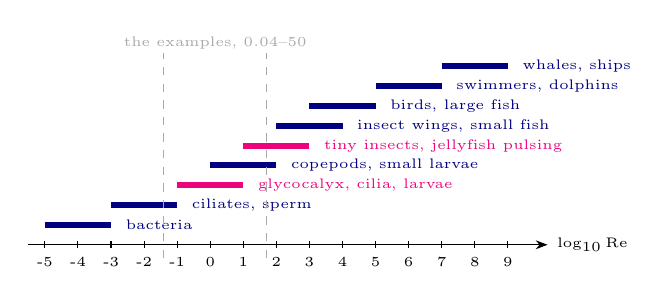
\begin{tikzpicture}[scale=0.42,every node/.style={font=\tiny}]
  \draw[-{Stealth[length=1.5mm]}] (-5.5,0) -- (10.2,0) node[right] {$\log_{10}\mathrm{Re}$};
  \foreach \x in {-5,-4,...,9}{\draw (\x,0.1) -- (\x,-0.1) node[below] {\x};}
  \foreach \lo/\hi/\y/\lab/\col in {-5/-3/0.6/bacteria/NavyBlue, -3/-1/1.2/{ciliates, sperm}/NavyBlue, -1/1/1.8/{glycocalyx, cilia, larvae}/RubineRed, 0/2/2.4/{copepods, small larvae}/NavyBlue, 1/3/3.0/{tiny insects, jellyfish pulsing}/RubineRed, 2/4/3.6/{insect wings, small fish}/NavyBlue, 3/5/4.2/{birds, large fish}/NavyBlue, 5/7/4.8/{swimmers, dolphins}/NavyBlue, 7/9/5.4/{whales, ships}/NavyBlue}{
    \draw[\col,line width=2.2pt] (\lo,\y) -- (\hi,\y);
    \node[anchor=west,text=\col] at (\hi+0.15,\y) {\lab};}
  \draw[dashed,DarkGray] (-1.4,-0.4) -- (-1.4,5.8); \draw[dashed,DarkGray] (1.7,-0.4) -- (1.7,5.8);
  \node[text=DarkGray] at (0.15,6.1) {the examples, $0.04$--$50$};
\end{tikzpicture}

\small Where the series' examples sit: the red bars. Everything biological from a ciliate to a bird is within six decades of them, which is why the same method serves for all of it; whales and ships are not.
\end{column}
\end{columns}
\end{frame}

% 12
\begin{frame}{Dimensionless time and frequency}
\label{fr:time}
\small ``For steady problems, time can be nondimensionalized as $t' = tU/L$. In applications with oscillating flows or motions, it is also important to think about the characteristic frequency: $f' = fL/U$. Be sure to match dimensionless frequency for pumping applications.'' (2018; the 2015 and 2020 versions say the same.)
\begin{itemize}
  \item $t'$ counts \al{advective times}: how many body lengths the stream has travelled. IB/03's ramp, $\tanh 2t$, is essentially over at $t = 1$ s, which is $t' = 1$; its run, $2$ s, is two body lengths of stream, and its drag coefficient is still settling at the end (slide \ref{fr:cd}).
  \item For a structure that moves on its own there is no $U$ until it moves; use the \al{viscous time} $L^2/\nu$ (IB/01: $\rho R^2/\mu = 0.12$ s, chapter 8a) or the elastic time $\sqrt{\rho L^3/K}$.
  \item $f'$ is the Strouhal number with $L$ as the length (next slide). IB/02: $f = 5$ Hz, $d = 1$ m, $U = 1$ m/s, so $f' = 5$: five pulses per advective time, a fast pulse; the fluid in the channel moves only $0.2$ m per cycle.
\end{itemize}
\vspace{1mm}
\begin{punchbox}
\footnotesize \code{END\_TIME} in these units: a start-up needs $t' \sim 1$--$3$ to settle (the leaf), a periodic flow needs several periods after the start-up (the channel: $0.25$ s is one and a quarter pulses, chapter 7's figure), and a creeping flow settles in a few viscous times. Choose the run length from the dimensionless clock, not from the wall clock.
\end{punchbox}
\end{frame}

% 13
\begin{frame}{The Strouhal number}
\label{fr:strouhal}
\small\setlength{\abovedisplayskip}{3pt}\setlength{\belowdisplayskip}{3pt} Two definitions, both in use; say which one you mean.
\[
  \mathrm{St}_L = \frac{fL}{U}, \qquad \mathrm{St}_A = \frac{fA}{U}.
\]
$\mathrm{St}_L$ is frequency times length over speed, the dimensionless frequency $f'$ of the previous slide; $\mathrm{St}_A$ uses the stroke amplitude $A$ instead of the body length.
\begin{itemize}\footnotesize
  \item From the 2018 lecture: ``A dimensionless parameter that describes the tail or wing kinematics of swimming and flying animals is the Strouhal number, $\mathrm{St} = fA/U$, which divides stroke frequency ($f$) and amplitude ($A$) by forward speed ($U$). St is known to govern a well-defined series of vortex growth and shedding regimes for airfoils undergoing pitching and heaving motions. Propulsive efficiency is high over a narrow range of St and usually peaks within the interval $0.2 < \mathrm{St} < 0.4$.'' (Taylor, Nudds and Thomas, \emph{Nature} 2003.)
  \item For vortex shedding from a cylinder, $\mathrm{St}_L = fD/U \approx 0.2$ over a wide range of $\mathrm{Re}$: the wake sets its own clock.
  \item ``In many biological applications, the frequency of vortex shedding equals the frequency of flapping (vortex shed during each direction change).'' (2014)
\end{itemize}
\begin{punchbox}
\footnotesize \al{Correction.} The 2014 ``What can go wrong'' slide wrote $\mathrm{St} = fU/L$. That is not dimensionless ($\mathrm{s}^{-1}\cdot\mathrm{m\,s^{-1}}/\mathrm{m} = \mathrm{s}^{-2}$); the number is $fL/U$. The 2018 and 2020 slides have it right.
\end{punchbox}
\end{frame}

% 14
\begin{frame}{Matching the frequency}
\label{fr:freq}
\small The 2014 recipe, ``The right frequency'': ``Let's say you are looking at oscillating flows or flapping. You calculate Re based on max velocity. What is the right flapping or pulsing frequency? Use dimensionless time, $t' = tU/L$. Calculate the correct dimensional time based on the application. Determine what your dimensional time should be to match that value.''
\begin{enumerate}
  \item Real animal: bell diameter $D$, pulse frequency $f$, swimming speed $U$. Compute $\mathrm{St}_L = fD/U$ (and $\mathrm{Re} = UD/\nu$).
  \item Simulation: choose $L_{\mathrm{sim}}$ and $U_{\mathrm{sim}}$ (unit scales, or the real ones). The simulated frequency must be $f_{\mathrm{sim}} = \mathrm{St}_L\,U_{\mathrm{sim}}/L_{\mathrm{sim}}$, and the viscosity $\mu_{\mathrm{sim}} = \rho_{\mathrm{sim}} U_{\mathrm{sim}} L_{\mathrm{sim}}/\mathrm{Re}$.
  \item The run must last the same number of periods as the comparison: $\mathrm{END\_TIME} = n/f_{\mathrm{sim}}$.
\end{enumerate}
\vspace{1mm}
\small Worked (slide \ref{fr:jelly}): a jellyfish with $D = 5$ cm, $f = 1$ Hz, $U = 5$ cm/s in water has $\mathrm{Re} = 2500$ and $\mathrm{St}_L = 1$. In unit scales ($L = U = \rho = 1$) that is $\mu = 4\times10^{-4}$ and $f = 1$, and ten pulses are \code{END\_TIME = 10}. In SI it is the animal itself, with $\mu = 10^{-3}$, and ten pulses are 10 s.
\vspace{1mm}

\small In IBAMR the frequency enters through a boundary condition (\code{sin(2*PI*f*t)}, chapter 7), a moving target (chapter 9a) or an active stress (IBFE/06): the same $f$ must appear in all of them.
\end{frame}

% 15
\begin{frame}{The Womersley number}
\label{fr:womersley}
\begin{columns}[T,onlytextwidth]
\begin{column}{0.6\textwidth}
\small\setlength{\abovedisplayskip}{2pt}\setlength{\belowdisplayskip}{1pt} For a flow that oscillates at angular frequency $\omega = 2\pi f$ in a vessel of radius $R$ (the 2018 slide quoted Wikipedia's definition and derivation):
\begin{gather*}
  \alpha = R\sqrt{\frac{\omega\rho}{\mu}} = R\sqrt{\frac{\omega}{\nu}} = \sqrt{2\pi\,\mathrm{Re}\,\mathrm{St}},\\
  \alpha^2 = \frac{\text{transient inertial force}}{\text{viscous force}}.
\end{gather*}
\begin{itemize}\footnotesize\setlength{\itemsep}{0pt}
  \item $\alpha \lesssim 1$: the viscous (Stokes) layer $\sqrt{\nu/\omega}$ fills the vessel; the profile is a quasi-steady parabola that follows the pressure gradient in phase.
  \item $\alpha \gg 1$: the layer is thin; the core moves as a plug and lags the pressure by up to $90^\circ$, and the peak velocity sits near the wall (the annular effect).
  \item ``The Womersley number is important in keeping dynamic similarity when scaling an experiment'' and ``in determining the thickness of the boundary layer to see if entrance effects can be ignored.''
\end{itemize}
\end{column}
\begin{column}{0.38\textwidth}
\footnotesize The three regimes in a channel of half-width $R$, with the Stokes layer $\delta = \sqrt{\nu/\omega}$ shaded:
\vspace{1mm}

\centering
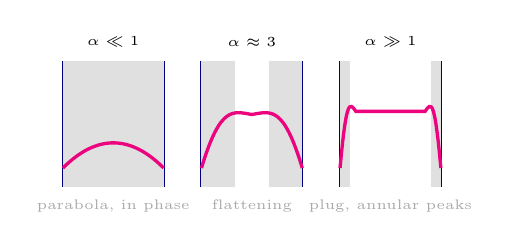
\begin{tikzpicture}[scale=0.8,every node/.style={font=\tiny}]
  \foreach \x/\lab/\d in {0/{$\alpha \ll 1$}/1.0, 2.2/{$\alpha \approx 3$}/0.33, 4.4/{$\alpha \gg 1$}/0.1}{
    \draw[NavyBlue,thick] (\x,0) -- (\x,2); \draw[NavyBlue,thick] (\x+1.6,0) -- (\x+1.6,2);
    \fill[LightGray!70] (\x,0) rectangle (\x+1.6*\d,2); \fill[LightGray!70] (\x+1.6-1.6*\d,0) rectangle (\x+1.6,2);
    \node at (\x+0.8,2.3) {\lab};}
  \draw[RubineRed,very thick] plot[domain=0:1.6,samples=30] (\x,{1.6*(\x/1.6)*(1-\x/1.6)+0.3});
  \draw[RubineRed,very thick] (2.2,0.3) .. controls (2.5,1.3) and (2.7,1.2) .. (3.0,1.15) -- (3.0,1.15) .. controls (3.3,1.2) and (3.5,1.3) .. (3.8,0.3);
  \draw[RubineRed,very thick] (4.4,0.3) .. controls (4.5,1.4) and (4.55,1.35) .. (4.65,1.2) -- (5.75,1.2) .. controls (5.85,1.35) and (5.9,1.4) .. (6.0,0.3);
  \node[text=DarkGray] at (0.8,-0.3) {parabola, in phase};
  \node[text=DarkGray] at (3.0,-0.3) {flattening};
  \node[text=DarkGray] at (5.2,-0.3) {plug, annular peaks};
\end{tikzpicture}
\end{column}
\end{columns}
\end{frame}

% 15b
\begin{frame}{Womersley numbers in a dog, and in the channel}
\label{fr:womersley2}
\begin{columns}[T,onlytextwidth]
\begin{column}{0.42\textwidth}
\scriptsize
\begin{tabular}{@{}L{0.5\textwidth}r@{}}
\toprule
Vessel (dog, heart rate 2 Hz) & $\alpha$\\
\midrule
ascending aorta & $13.2$\\
descending aorta & $11.5$\\
abdominal aorta & $8.0$\\
femoral artery & $3.5$\\
carotid artery & $4.4$\\
arterioles & $0.04$\\
capillaries & $0.005$\\
venules & $0.035$\\
inferior vena cava & $8.8$\\
main pulmonary artery & $15$\\
\bottomrule
\end{tabular}

\vspace{1mm}
\scriptsize The 2018 slide's table (Wikipedia, ``Womersley number''); the theory deck checks the aorta value from the radius and the viscosity of blood.
\end{column}
\begin{column}{0.56\textwidth}
\small
\begin{itemize}
  \item The aorta at $\alpha = 13$ is a plug flow with thin wall layers; the capillaries at $0.005$ are quasi-steady Poiseuille flow that follows the pressure in phase. A model of either must reproduce its $\alpha$, which fixes $f$ once $R$ and $\nu$ are chosen.
  \item IB/02: $R = 0.5$ m, $f = 5$ Hz, $\nu = 0.1$ m$^2$/s: $\alpha = 0.5\sqrt{31.4/0.1} = 8.9$, aorta-like. Chapter 7's figure of the channel at a trough shows the annular effect that this predicts: the core has stopped while the layers near the walls still move.
  \item With $\mathrm{Re} = 10$ and $\mathrm{St} = 5$, $\sqrt{2\pi\times10\times5} = 17.7$ with the full width; with the half-width $R$ it is $8.9$, as computed. Say which length the number uses.
  \item To lower $\alpha$ in IB/02 without changing $\mathrm{Re}$, lower $f$: at $f = 0.1$ Hz, $\alpha = 1.25$ and the profile is a parabola throughout the cycle.
\end{itemize}
\end{column}
\end{columns}
\end{frame}

% 16
\begin{frame}{The P\'eclet number}
\label{fr:peclet}
\small For a scalar (heat, a chemical, a dye) carried by the flow and diffusing with diffusivity $D$ (the 2018 slide quoted Wikipedia):
\[
  \mathrm{Pe} = \frac{\text{advective transport rate}}{\text{diffusive transport rate}} = \frac{UL}{D} = \mathrm{Re}\,\mathrm{Sc}, \qquad \mathrm{Sc} = \frac{\nu}{D}\ \text{(Schmidt; Prandtl for heat)}.
\]
\begin{itemize}
  \item $\mathrm{Pe} \gg 1$: the scalar is swept along as a tracer and its fronts stay sharp (and need a fine grid); $\mathrm{Pe} \ll 1$: it diffuses faster than the flow moves it and fills the domain.
  \item IBFE/12 (chapter 15): $U = 0.5$, $L = 1$, \code{KAPPA = 1.0e-6}, so $\mathrm{Pe} = 5\times10^5$: the temperature field is a passive marker of where the fluid went, and its diffusion is negligible over the run.
  \item Biology: oxygen in water, $D \approx 2\times10^{-9}$ m$^2$/s, so $\mathrm{Sc} \approx 500$ and a larva at $\mathrm{Re} = 1$ has $\mathrm{Pe} \approx 500$; a chemical signal around a sponge or a coral is advection-dominated as soon as the flow moves at all.
\end{itemize}
\vspace{1mm}
\begin{punchbox}
\small Matching $\mathrm{Re}$ does not match $\mathrm{Pe}$: with $D$ fixed by the chemistry, changing $\nu$ to set $\mathrm{Re}$ changes $\mathrm{Sc}$. A dimensionless advection--diffusion run must set $D_{\mathrm{sim}} = U_{\mathrm{sim}}L_{\mathrm{sim}}/\mathrm{Pe}$ separately.
\end{punchbox}
\end{frame}

% 17
\begin{frame}{Dimensionless force per unit length}
\label{fr:force}
\small The 2018/2020 text: ``You might apply a force to a 1D fiber before it is spread to the fluid. This gives you a force per unit length. To nondimensionalize it:
$F' = F/(\rho L U^2)$ for $\mathrm{Re} > 1$, $F' = F/(\mu U)$ for $\mathrm{Re} < 1$.''
\begin{itemize}
  \item In the theory deck's words: a force resultant per unit depth $\mathcal{F}$ (N/m) has the inertial scale $\mathcal{F}_I = \rho U^2 L$ and the viscous scale $\mathcal{F}_V = \mu U$, and $\mathcal{F}/\mathcal{F}_V = \mathrm{Re}\;\mathcal{F}/\mathcal{F}_I$. There is no switch at $\mathrm{Re} = 1$; the two are the same number in different units.
  \item A Lagrangian force density along a fibre (force per unit length of fibre per unit depth, N/m$^2$ in 2D) scales as $\rho U^2$ or $\mu U/L$; the \emph{total} force on a body of size $L$ is that times $L$.
  \item IBAMR's \code{integral\{F\}} (chapter 11) is the total Lagrangian force: in 2D a force per unit depth, in 3D a force. Divide by $\rho U^2 L$ (2D) or $\rho U^2 L^2$ (3D) for the inertial coefficient, by $\mu U$ or $\mu U L$ for the viscous one.
\end{itemize}
\vspace{1mm}
\begin{punchbox}
\small Conventions differ by a factor $2$: the aerodynamic coefficients (next slide) divide by $\frac12\rho U^2$, the course's scale by $\rho U^2$. Both are fine; state which, and the length used.
\end{punchbox}
\end{frame}

% 18
\begin{frame}{Drag and lift coefficients}
\label{fr:cdcl}
\begin{columns}[T,onlytextwidth]
\begin{column}{0.54\textwidth}
\footnotesize For $\mathrm{Re} \gg 1$ (the 2018 ``Dimensions continued'' slide):
\[
  C_L = \frac{2F_L}{\rho U^2 S}, \qquad C_D = \frac{2F_D}{\rho U^2 S},
\]
``where $S$ is the surface area per unit length of the structure, $U$ is the velocity of the boundary, $F_D$ is the drag force per unit length, $F_L$ the lift force per unit length.'' In 2D, per unit depth, $S$ becomes the projected length $L$ of the object normal to the flow and $F$ a force per unit depth (N/m); in 3D, $S$ is the projected (or planform) area and $F$ a force.
\begin{itemize}
  \item Drag: the force along the flow; lift: the force across it. Both are the total fluid force on the body, which in an IB simulation is minus the total Lagrangian force (next slide).
  \item The lift coefficient of an aerofoil rises linearly with the angle of attack ($\approx 2\pi\alpha$ in thin-aerofoil theory) up to stall at $15$--$20^\circ$; the 2018 slide showed Wikipedia's $C_L(\alpha)$ plot.
\end{itemize}
\end{column}
\begin{column}{0.44\textwidth}
\scriptsize
\begin{tabular}{@{}L{0.5\textwidth}r@{}}
\toprule
Shape ($\mathrm{Re} \sim 10^4$) & $C_D$\\
\midrule
sphere & $0.47$\\
half-sphere & $0.42$\\
cone & $0.50$\\
cube & $1.05$\\
angled cube & $0.80$\\
long cylinder & $0.82$\\
short cylinder & $1.15$\\
streamlined body & $0.04$\\
streamlined half-body & $0.09$\\
\midrule
flat plate normal to the flow, 2D & $\approx 2$\\
the same at $\mathrm{Re} = 2.5$ (IB/03, measured) & $9.4$\\
\bottomrule
\end{tabular}

\vspace{1mm}
\scriptsize Measured drag coefficients as tabulated on Wikipedia, ``Drag coefficient'' (the 2018 slide's figure), plus the two plate values. At low $\mathrm{Re}$ the coefficient grows as $1/\mathrm{Re}$ because the force is viscous, $\propto \mu U$, not $\rho U^2$.
\end{column}
\end{columns}
\end{frame}

% 19
\begin{frame}{A drag coefficient from an IBAMR run: the leaf}
\label{fr:cd}
\begin{columns}[T,onlytextwidth]
\begin{column}{0.58\textwidth}
\centering
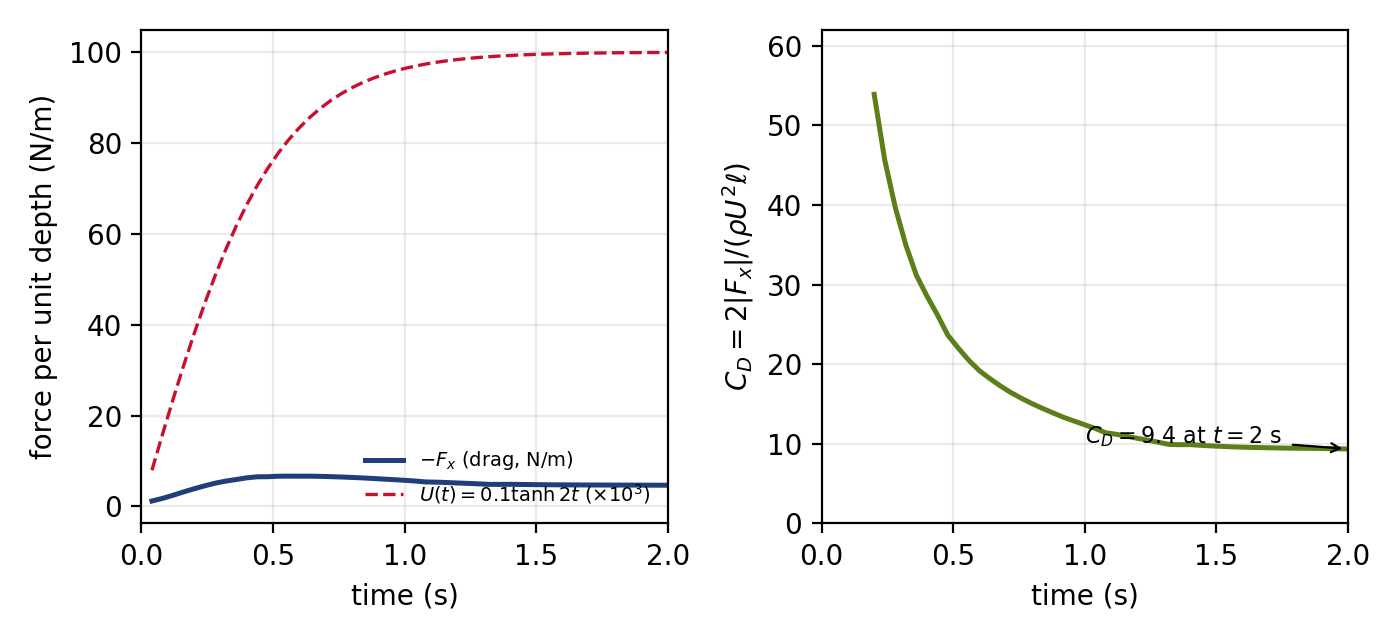
\includegraphics[width=\textwidth]{ch8b-leaf-cd}
\end{column}
\begin{column}{0.4\textwidth}
\footnotesize IB/03 prints \code{integral\{F\}} every $0.04$ s: the sum of all Lagrangian forces, which is the target force holding the leaf, equal and opposite to the drag of the stream (README). At $t = 2$ s it is $-4.67$ N/m.
\begin{itemize}
  \item $C_D = 2|F_x|/(\rho U^2\ell)$ with $U = 0.1\tanh 2t$ and $\ell = 0.1$ m: $9.4$ at $t = 2$ s, still falling slowly ($9.7$ at $1.5$ s, $12.4$ at $1$ s).
  \item Left: the force (solid) and the stream speed (dashed); right: the coefficient from $t = 0.2$ s on.
\end{itemize}
\end{column}
\end{columns}
\sourcecredit{IB/03 shipped run, IBAMR 0.19.0; \code{tools/ch8b\_figures.py} reads the 50 \code{integral\{F\}} lines of \code{run.log}. The early points ($t < 0.2$ s) are left out of the coefficient: $U$ is near zero there and the ratio is meaningless.}
\end{frame}

% 19b
\begin{frame}{Reading the drag curve}
\label{fr:cd2}
\footnotesize
\begin{itemize}
  \item The force \al{peaks} at $t \approx 0.5$--$0.7$ s ($6.6$ N/m) while the stream is still accelerating: part of it is the acceleration reaction (added mass, a force $\propto \rho\ell^2\,dU/dt$ per depth), part the drag of a leaf not yet bent out of the way. That is the same overshoot as the tip displacement of chapter 8a, seen in the force.
  \item After the ramp the force falls as the leaf bends and the wake forms, and the coefficient falls with it: $C_D(t)$ is not a constant until the flow is steady, which at $t' = 2$ it nearly is. A drag coefficient quoted from a start-up run must say at what $t'$ it was taken.
  \item $C_D \approx 9$ for a plate normal to the flow at $\mathrm{Re} = 2.5$ is reasonable: a circular cylinder at $\mathrm{Re} = 2.5$ has $C_D \approx 8$, and the coefficient grows as $1/\mathrm{Re}$ below $\mathrm{Re} \sim 100$ because the force is viscous there.
  \item The viscous scaling says the same thing: $F/(\mu U) = 4.67/(4\times0.1) = 11.7$, and $\mathrm{Re}\,C_D/2 = 2.5\times9.4/2 = 11.7$; the two coefficients are the same number in different units (slide \ref{fr:force}).
\end{itemize}
\vspace{1mm}
\begin{punchbox}
\small The whole computation is four lines of Python on \code{run.log}; chapter 11 does the same for the point-by-point forces and for lift. Report it as ``$C_D = 9.4$ at $\mathrm{Re} = 2.5$ (leaf length, free-stream speed, $t' = 2$, $\frac12$ convention)''.
\end{punchbox}
\end{frame}

% 20
\begin{frame}{What is the beam stiffness? Young's modulus and the second moment of area}
\label{fr:ei}
\begin{columns}[T,onlytextwidth]
\begin{column}{0.5\textwidth}
\small ``This is equivalent to the flexural rigidity. The flexural rigidity in 3D has units N m$^2$, and is given by $EI$, where $E$ is the elastic or Young's modulus (N/m$^2$) and $I$ is the second moment of area (in units of length$^4$). The flexural rigidity in 2D has units N m.'' (2018/2020)
\begin{itemize}
  \item $I = \int_A y^2\,dA$ about the bending axis. A rectangle of base $b$ and height $h$: $I = bh^3/12$. A circle of radius $r$: $\pi r^4/4$. A thin plate bends about its thin dimension, so $h$ is the thickness.
  \item Per unit depth (2D): $EI/b = Eh^3/12$, in N m.
  \item Stiffness grows as the \emph{cube} of the thickness: doubling a leaf's thickness makes it eight times stiffer.
\end{itemize}
\end{column}
\begin{column}{0.48\textwidth}
\scriptsize
\begin{tabular}{@{}L{0.52\textwidth}r@{}}
\toprule
Material & $E$ (GPa)\\
\midrule
rubber (small strain) & $0.01$--$0.1$\\
low-density polyethylene & $0.11$--$0.45$\\
diatom frustules (silicic acid) & $0.35$--$2.8$\\
PTFE (Teflon) & $0.5$\\
polypropylene & $1.5$--$2$\\
nylon & $2$--$4$\\
oak wood (along the grain) & $11$\\
human cortical bone & $14$\\
aluminium & $69$\\
tooth enamel & $83$\\
\bottomrule
\end{tabular}

\vspace{1mm}
\scriptsize From the table the 2018 slide reproduced (Wikipedia, ``Young's modulus''). Plant leaves and soft tissues are $10^{-3}$ to $10^{-1}$ GPa; a jellyfish mesoglea $10^{-5}$ GPa.
\end{column}
\end{columns}
\end{frame}

% 21
\begin{frame}{Dimensionless bending coefficient, and the thresholds reconciled}
\label{fr:kbeam}
\small ``Note that $k_{\mathrm{beam}}$ in 2D is assumed to have units of N m.'' (2018)
\[
  \text{2D, } \mathrm{Re} > 1:\quad k'_{\mathrm{beam}} = \frac{k_{\mathrm{beam}}}{\rho U^2 L^3}, \qquad
  \text{2D, } \mathrm{Re} < 1:\quad k'_{\mathrm{beam}} = \frac{k_{\mathrm{beam}}}{\mu U L^2}, \qquad
  \text{3D:}\quad \frac{EI}{\rho U^2 L^4}.
\]
\begin{itemize}
  \item The denominators are bending-moment scales: a pressure ($\rho U^2$ or $\mu U/L$) over a length $L$, times a lever arm $L$, times the width (unit depth in 2D, $L$ in 3D). The viscous and inertial forms differ by $\mathrm{Re}$: $k'^{(V)} = \mathrm{Re}\,k'^{(I)}$.
  \item The 2014 slides wrote $L^4$ in 2D: a units slip ($L^4$ is the 3D form); the 2015, 2018 and 2020 slides have $L^3$. Chapter 8a's estimate slide uses $L^3$.
\end{itemize}
\vspace{1mm}
\begin{punchbox}
\small \al{The ``little bending'' threshold} was $k' = 1$ (2014), $1$--$10$ (2018) and $10$ (2015, 2017, 2020), each ``typically resulting in a little bit of bending (maybe 2--10 degrees)''. The theory deck calls the number ``a model-specific starting guess, not a universal relation''. Chapter 8a measured it on the leaf: $k' = 5$ gives about $1^\circ$, $0.5$ gives $10$--$16^\circ$, $0.05$ folds over. So on that model ``a few degrees'' is $k' \approx 2$--$5$, and all three old values are within the right decade.
\end{punchbox}
\end{frame}

% 22
\begin{frame}{Dimensionless stretching coefficient}
\label{fr:kspring}
\small ``Note that $k_{\mathrm{spring}}$ is assumed to have units of N/m.'' (2018)
\[
  \text{2D, } \mathrm{Re} > 1:\quad k'_{\mathrm{spring}} = \frac{k_{\mathrm{spring}}}{\rho U^2 L}, \qquad
  \text{2D, } \mathrm{Re} < 1:\quad k'_{\mathrm{spring}} = \frac{k_{\mathrm{spring}}}{\mu U}.
\]
\begin{itemize}\footnotesize
  \item Here $k_{\mathrm{spring}}$ is the \al{tension per unit strain} of the fibre per unit depth, $K$ in chapter 6's notation (N/m in 2D): the generator's \code{kappa\_spring}, not the file value $K/\Delta s$. With $K$ the force per unit strain, $k'$ compares the tension at unit strain with the fluid's force scale $\rho U^2 L$; $k' \gg 1$ means the fibre is effectively inextensible under the flow.
  \item IB/03: $K = 30$, so $k' = 30/(1000\times0.01\times0.1) = 30$: the leaf stretches by at most a few per cent (it does not, visibly).
  \item IB/01: $K = 2000$ in creeping flow, $k'^{(V)} = 2000/(100\times0.02) = 1000$: the band is inextensible as far as the fluid is concerned; it stays $9.5\%$ stretched only because the enclosed area forces it to (chapter 8a).
  \item IB/06: the springs are the \emph{drive}; their rest length grows and $k' = 2000/(100\times0.5) = 40$ in the viscous scaling with the fibre's end speed $0.5$ m/s.
\end{itemize}
\footnotesize The theory deck's caution applies: ``a point-spring stiffness and three-dimensional line, surface, or volume coefficients have different units. Begin with the exact force law and integration measure.'' The next two slides do exactly that for IBAMR.
\end{frame}

% 23
\begin{frame}[fragile]{Where IBAMR's spring stiffness comes from}
\label{fr:springlaw}
\begin{columns}[T,onlytextwidth]
\begin{column}{0.5\textwidth}
\scriptsize The 2018 ``Dimensions continued'' deck derived it in three steps (its slides 5--7, which were screenshots of lecture notes):
\begin{enumerate}
  \item \al{Energy.} Points $m$ and $n$ joined by a linear spring of stiffness $k_{\mathrm{sp}}$ and rest length $l_s$ have $E_S = \tfrac12 k_{\mathrm{sp}}\,(|\mathbf{X}_m - \mathbf{X}_n| - l_s)^2$; the force on each point is minus its gradient.
  \item \al{Tension.} For a continuous fibre $\mathbf{X}(s)$, the tension is $T = \sigma(|\partial\mathbf{X}/\partial s|)$, the unit tangent $\boldsymbol{\tau} = (\partial\mathbf{X}/\partial s)/|\partial\mathbf{X}/\partial s|$, and the force density $\mathbf{f} = \partial(T\boldsymbol{\tau})/\partial s$ (Peskin 2002).
  \item \al{Discretization.} ``Examining the equation for $\mathbf{f}$ illustrates how the calculation of force would yield $(\partial s/\partial s)/\partial s$, where $\partial s/\partial s$ comes from the calculation of $\boldsymbol{\tau}$, and $1/\partial s$ from $\partial(T\boldsymbol{\tau})/\partial s$. In IBAMR, $(\partial s/\partial s)/\partial s$ is not explicitly calculated and gets lumped into the \code{kappa\_spring} term.''
\end{enumerate}
\begin{lstlisting}[style=matlabtiny]
for s = 0:npts-2
   fprintf(spring_fid, '%d %d %1.16e %1.16e\n', s, s+1, kappa_spring*ds/(ds^2), ds);
end
\end{lstlisting}
\end{column}
\begin{column}{0.48\textwidth}
\scriptsize So the file holds $K\,\Delta s/\Delta s^2 = K/\Delta s$ (chapter 6), and the force between two points is linear in the stretch:
\[
  \mathbf{F}_{m} = \frac{K}{\Delta s}\,\bigl(|\mathbf{X}_n - \mathbf{X}_m| - l_s\bigr)\,\frac{\mathbf{X}_n - \mathbf{X}_m}{|\mathbf{X}_n - \mathbf{X}_m|},
\]
and $\mathbf{F}_n = -\mathbf{F}_m$.
With $l_s = \Delta s$ and a stretch $\epsilon = (|\mathbf{X}_n - \mathbf{X}_m| - \Delta s)/\Delta s$ this is $K\epsilon$: \al{tension $=$ $K$ times strain}, the continuum law, on every segment. That is why $K$, not the file value, is the physical stiffness and the one that goes into $k'_{\mathrm{spring}}$.
\scriptsize The sum over a fibre's segments of $\mathbf{F}_m$ is the discrete $\partial(T\boldsymbol{\tau})/\partial s$ times $\Delta s$: a force per point, which the kernel spreads over $\Delta x^{\mathrm{dim}}$ to give the Eulerian force density $\mathbf{F}$ of slide \ref{fr:ns}.
\end{column}
\end{columns}
\end{frame}

% 24
\begin{frame}[fragile]{The same law in the 0.19.0 source}
\label{fr:springcode}
\begin{columns}[T,onlytextwidth]
\begin{column}{0.56\textwidth}
\begin{lstlisting}[style=cpptiny]
// src/IB/IBStandardForceGen.cpp, computeLagrangianSpringForce (condensed)
D[0] = X_node[slave_idx + 0] - X_node[mastr_idx + 0];   // X_n - X_m
D[1] = X_node[slave_idx + 1] - X_node[mastr_idx + 1];
R = std::sqrt(D[0] * D[0] + D[1] * D[1]);               // |X_n - X_m|
T_over_R = (force_fcns[k])(R, parameters[k], lag_mastr_node_idxs[k], lag_slave_node_idxs[k]) / R;
F[0] = T_over_R * D[0];                                 // tension along the spring
F[1] = T_over_R * D[1];
F_node[mastr_idx + 0] += F[0];                          // on the first point ...
F_node[mastr_idx + 1] += F[1];
F_node[slave_idx + 0] -= F[0];                          // ... and minus it on the second
F_node[slave_idx + 1] -= F[1];
\end{lstlisting}
\footnotesize The 2018 slide showed a screenshot of this routine from the then-current GitHub master; the 2D lines above are the 0.19.0 version. \code{force\_fcns[k]} is the spring's force function: by default $T(R) = \kappa\,(R - l_s)$ with $\kappa$ and $l_s$ the file's two numbers (\code{parameters[k][0]}, \code{[1]}); chapter 9b replaces it with your own.
\end{column}
\begin{column}{0.42\textwidth}
\footnotesize What to read off:
\begin{itemize}
  \item the tension is a scalar function of the length $R$ alone, times the unit vector $\mathbf{D}/R$: a central force;
  \item the file's $\kappa$ multiplies a \emph{length} and returns a \emph{force on a point}, so its units are N/m (3D) or N/m$^2$ (2D per depth), which is $K/\Delta s$;
  \item nothing in the code knows $\Delta s$: the generator must put it in. Refine the grid without regenerating and $K/\Delta s$ is the old one (chapter 8a);
  \item the beam force is assembled the same way from the second difference of three points, with $EI/\Delta s^3$ as its coefficient (chapter 6).
\end{itemize}
\end{column}
\end{columns}
\end{frame}

% 25
\begin{frame}{The IB equations with their units}
\label{fr:ibunits}
\footnotesize The 2018 deck closed with the equations in dimensional form (screenshots of Peskin's chapter); typeset here with the units that the 2D ``per unit depth'' convention implies.
\begingroup\footnotesize
\begin{align*}
  \rho\Bigl(\frac{\partial\mathbf{u}}{\partial t} + \mathbf{u}\cdot\nabla\mathbf{u}\Bigr) &= -\nabla p + \mu\nabla^2\mathbf{u} + \mathbf{F}, \quad \nabla\cdot\mathbf{u} = 0, & [\mathbf{F}] &= \mathrm{N/m^3}\ (3\mathrm{D});\ \mathrm{N/m^2}\ \text{per depth}\ (2\mathrm{D})\\
  \mathbf{F}(\mathbf{x},t) &= \int \mathbf{f}(s,t)\,\delta\bigl(\mathbf{x} - \mathbf{X}(s,t)\bigr)\,ds, & [\mathbf{f}] &= \mathrm{N/m}\ \text{per length of fibre, per depth}\\
  \frac{\partial\mathbf{X}}{\partial t}(s,t) &= \mathbf{u}\bigl(\mathbf{X}(s,t),t\bigr) = \int \mathbf{u}(\mathbf{x},t)\,\delta\bigl(\mathbf{x} - \mathbf{X}(s,t)\bigr)\,d\mathbf{x}, & [\delta] &= \mathrm{m}^{-\mathrm{dim}}\\
  \mathbf{f}(s,t) &= \frac{\partial}{\partial s}\bigl(T\boldsymbol{\tau}\bigr) - \frac{\partial^2}{\partial s^2}\Bigl(EI\,\frac{\partial^2\mathbf{X}}{\partial s^2}\Bigr) + \ldots & [T] &= \mathrm{N}\ \text{per depth};\ [EI] = \mathrm{N\,m}\ \text{per depth}.
\end{align*}
\endgroup
\begin{itemize}\footnotesize
  \item ``Note that $\mathbf{f}$ is a force density'': in 3D with two Lagrangian parameters $(q,r,s)$ it is a force per unit volume of the Lagrangian coordinate space, and $\mathbf{F}$ is N/m$^3$; in 2D with one parameter it is force per unit length (per unit depth) and $\mathbf{F}$ is N/m$^2$ (per unit depth). The $\delta$ function carries the remaining m$^{-\mathrm{dim}}$.
  \item Non-dimensionalize with $\mathbf{F} = (\rho U^2/L)\,\mathbf{F}'$, $\mathbf{f} = \rho U^2\,\mathbf{f}'$ (2D), $T = \rho U^2 L\,T'$, $EI = \rho U^2 L^3\,(EI)'$: the primes are exactly $k'_{\mathrm{spring}}$ and $k'_{\mathrm{beam}}$ of slides \ref{fr:kbeam}--\ref{fr:kspring}.
\end{itemize}
\footnotesize The derivation of the interaction equations and their discretization are chapter 5 and the theory series' Module 1-2.
\end{frame}

% 26
\begin{frame}[fragile]{Worked example: a velocity for growing springs (IB/06)}
\label{fr:growing}
\begin{columns}[T,onlytextwidth]
\begin{column}{0.5\textwidth}
\scriptsize The 2018 exercise on \code{Example\_2DUpdateSprings} (now IB/06, chapter 9a): ``the resting length is being changed at each time step, \code{resting\_length += 0.01*dt}. $0.01\,dt$ is a change in displacement equal to a velocity ($0.01$) times a change in time. $0.01$ is the velocity of the resting length of one spring. Note that these springs are in series: the velocity of the resting length of the entire plate is \code{npts}$\,\times\,0.01$.''
\vspace{1mm}

\scriptsize ``Determine a reasonable maximum velocity. $dx = L/512 = 1/512$, $ds = dx/2 = 1/1024$. The length of the plate is $0.1$, so \code{npts} $\approx 102$. If we want the plate to change its total resting length by $0.05$ m/s (it would get 50\% longer in 1 second), then $V_{\mathrm{spring}} = V_{\mathrm{plate}}/\mathrm{npts} = 0.05/102 = 0.00049$.''
\vspace{1mm}

\scriptsize ``Make the velocity vary in time: multiply by $\sin(2\pi f t)$; with $f = 1$ Hz the velocity oscillates between $\pm0.00049$.''
\end{column}
\begin{column}{0.48\textwidth}
\begin{lstlisting}[style=cpptiny]
// original (2018 exercise)
resting_length += 0.01*dt;
// modified: a velocity of a single spring, times the change in time
resting_length += 0.00049*sin(2*pi*current_time)*dt;
\end{lstlisting}
\begin{lstlisting}[style=cpptiny]
// IB/06 update_springs.cpp as shipped (0.19.0 API, chapter 9a)
static const double growth_rate = 0.01;   // how fast each rest length grows (m/s)
...
spring[1] += growth_rate * dt;             // spring[1] is the rest length
\end{lstlisting}
\scriptsize The dimensional reasoning is the point: a rate per spring becomes a rate for the whole fibre by the number of springs in series, and ``$0.01$'' only means something once its units (m/s per spring) are written down. With the shipped rate the 102 springs lengthen the fibre by $1.02$ m/s: by $t = 0.5$ s the rest lengths add up to $0.61$ m (README), five times the starting length, which is why the series runs it for $0.5$ s and not the course's 2 s.
\scriptsize Dimensionless: the growth speed over the fibre length is a frequency; $f' = (1.02/0.1)\times(0.1/0.5)$ with the fibre's own end speed as $U$, i.e.\ $\mathrm{St}_L \approx 2$.
\end{column}
\end{columns}
\end{frame}

% 27
\begin{frame}{More than matching Re}
\label{fr:matchall}
\footnotesize The 2014 lecture: ``As mathematicians, we may not think about real units very much. You can match Re, but is that good enough? Not always; there are other dimensionless numbers to match: dimensionless bending and stretching stiffness, Strouhal number (flapping frequency, pumping frequency).'' The full list for an IB model:

\tiny
\begin{tabular}{@{}L{0.2\textwidth}L{0.26\textwidth}L{0.44\textwidth}@{}}
\toprule
Group & definition & when it matters\\
\midrule
Reynolds & $\rho UL/\mu$ & always\\
Strouhal (frequency) & $fL/U$, $fA/U$ & any periodic motion or inflow: flapping, pulsing, pumping, shedding\\
Womersley & $R\sqrt{\omega\rho/\mu}$ & oscillating flow in a channel or vessel (it is $\sqrt{2\pi\,\mathrm{Re}\,\mathrm{St}}$, so it follows from the two above)\\
bending coefficient & $EI/(\rho U^2L^3)$ (2D) & any flexible structure; the Cauchy number is its inverse\\
stretching coefficient & $K/(\rho U^2 L)$ & any extensible fibre; $\gg 1$ means inextensible\\
tether stiffness & $\kappa L/(\rho U^2)$ or similar & prescribed motion by target points: how closely the targets are followed (chapter 9a)\\
P\'eclet & $UL/D$ & any transported scalar (chapter 15)\\
density ratio & $\rho_s/\rho$ & only with added mass (chapter 13); IB structures are massless, $\rho_s/\rho = 1$\\
geometry & $L_{\mathrm{box}}/L$, aspect ratios, gap/$L$ & always: the box must not be part of the physics\\
Froude & $U/\sqrt{gL}$ & only with gravity and a free surface; none of the examples\\
\bottomrule
\end{tabular}

\footnotesize ``Be safe: match all numbers to reality.'' If a group cannot be matched (a $10^{-3}$ Pa s fluid at $\mathrm{Re} = 10^5$ in 2D), say which one was sacrificed and why.
\end{frame}

% 28
\begin{frame}{The examples' dimensionless numbers}
\label{fr:extable}
\tiny
\setlength{\tabcolsep}{3pt}
\begin{tabular}{@{}L{0.17\textwidth}cL{0.17\textwidth}L{0.2\textwidth}L{0.14\textwidth}L{0.14\textwidth}@{}}
\toprule
example & $\mathrm{Re}$ & frequency / St & bending $k'_{\mathrm{beam}}$ & stretching $k'_{\mathrm{spring}}$ & box / body\\
\midrule
IB/01 band & $0.04$ & none imposed; swing period $0.3$ s at $\mu \le 10$ & -- & $1000$ (viscous) & $5$\\
IB/02 channel & $10$ & $f' = 5$; $\alpha = 8.9$ & -- & walls: targets & $5$\\
IB/03 leaf & $2.5$ & ramp over $t' = 1$ & $0.5$ ($1.25$ viscous) & $30$ & $10$\\
IB/04 cylinders & $0.01$ & speed ramp $0.1$ s & -- & targets & $200$ (gap/$D$ = 9)\\
IB/06 growing fibre & $0.5$ & $\mathrm{St}_L \approx 2$ & -- & $40$ (viscous) & $10$\\
IB/07 plates & $0.2$ & speed ramp $0.1$ s & $0.125$ ($0.025$ viscous) & $100$ (viscous) & $10$ (gap/$L$ = 0.05)\\
IB/08 glycocalyx (3D) & $0.061$ & lid ramp $\tanh 2t$ & -- & targets & $5$ across, $6$ tall\\
IBFE/01, 05, 12 plates & $50$ & tether 1 s up, 2 s down & $\mu_s/(\rho U^2) = 40$ & -- & $2$ (periodic)\\
IBFE/06 active plate & its own & \code{FIBER\_MODE} & $\mu_s/(\rho U^2)$, $U$ from the contraction & -- & $2$\\
IBFE/08 plate and disc & $25$ & tether $0.25$ for 1 s & $160$ & -- & $4$\\
IBFE/10 tank (3D) & $20$ & stream ramp & $\mu_s/(\rho U^2)$ with $\beta\ln J$ & -- & $16 \times 8 \times 8$\\
\bottomrule
\end{tabular}

\footnotesize For the IBFE solids the stiffness group is the shear modulus over the dynamic pressure, $\mu_s/(\rho U^2)$ (its inverse is the Cauchy number): IBFE/01 has $10/(1\times0.25) = 40$, IBFE/08 $10/(1\times0.0625) = 160$. ``Targets'' means the structure is held by target points and the stiffness group is the tether one (chapter 9a). Every number is from the input files and READMEs; the Reynolds numbers are chapter 8a's.
\end{frame}

% 29
\begin{frame}{Worked conversion 1: a jellyfish}
\label{fr:jelly}
\small A small jellyfish: bell diameter $D = 5$ cm, pulse frequency $f = 1$ Hz, swimming speed $U = 5$ cm/s, in sea water ($\rho = 1025$ kg/m$^3$, $\nu = 10^{-6}$ m$^2$/s).
\begin{columns}[T,onlytextwidth]
\begin{column}{0.5\textwidth}
\footnotesize
\begin{tabular}{@{}L{0.3\textwidth}L{0.6\textwidth}@{}}
\toprule
group & value\\
\midrule
$\mathrm{Re} = UD/\nu$ & $0.05\times0.05/10^{-6} = 2500$\\
$\mathrm{St}_L = fD/U$ & $1\times0.05/0.05 = 1$\\
$\alpha$ (bell as the vessel) & $0.025\sqrt{2\pi/10^{-6}} = 63$\\
bell stiffness & mesoglea $E \sim 10^4$ Pa, thickness $h \sim 5$ mm: $EI/b = Eh^3/12 \approx 10^{-4}$ N m; $k' = 10^{-4}/(1025\times0.0025\times1.25\times10^{-4}) \approx 0.3$\\
\bottomrule
\end{tabular}

\vspace{1mm}
\footnotesize (The bell's stiffness is an order of magnitude only: real mesoglea is layered and the muscle sets the shape.)
\end{column}
\begin{column}{0.48\textwidth}
\footnotesize \al{In unit scales} ($\rho = L = U = 1$): \code{MU = 1/2500}, the pulse \code{sin(2*PI*1*t)} in the active force, $k_{\mathrm{beam}} = 0.3$, a box of $10$, \code{END\_TIME = 10} for ten pulses, a grid fine enough for a boundary layer of $D/\sqrt{\mathrm{Re}} = 0.02$ (so $\Delta x \le 0.005$, $2000$ cells across the box, four levels of refinement).
\vspace{1mm}

\footnotesize \al{In SI}: the animal as is, $\mu = 10^{-3}$, $D = 0.05$, $f = 1$, $k_{\mathrm{beam}} = 10^{-4}$, a $0.5$ m box, 10 s. Same numbers, same run.
\vspace{1mm}

\footnotesize \al{What the examples lack}: IB/03 is at $\mathrm{Re} = 2.5$, a thousand times lower; a jellyfish run is a $\mathrm{Re} = 2500$ run, with the resolution and the time step that implies (chapters 5, 16). The 2016 jellyfish models in the archive (Part X) were set up this way.
\end{column}
\end{columns}
\end{frame}

% 30
\begin{frame}{Worked conversion 2: the leaf, as a leaf}
\label{fr:leafreal}
\small IB/03 is a ``leaf'' $0.1$ m long in a fluid of viscosity $4$ Pa s at $0.1$ m/s: $\mathrm{Re} = 2.5$. A real leaf in a breeze: $\ell = 0.1$ m, $U = 1$ m/s, air ($\rho = 1.2$, $\nu = 1.5\times10^{-5}$).
\begin{itemize}
  \item $\mathrm{Re} = 1\times0.1/1.5\times10^{-5} \approx 6700$: nearly three decades above the model. The model is a leaf in syrup, chosen so that the course's first flexible-body run resolves everything on a $512^2$ grid.
  \item To run the real leaf in the same SI box: $\mu = \rho U\ell/\mathrm{Re}$ with the model's $\rho = 1000$ and $U = 0.1$ gives $\mu = 1.5\times10^{-3}$ Pa s, water. The boundary layer, $\ell/\sqrt{\mathrm{Re}} = 1.2$ mm, is $0.6\,\Delta x$ at $N = 512$: under-resolved. Four times the grid and a quarter of \code{DT} are the price (chapter 7's grid rules, chapter 16).
  \item The stiffness: a leaf of thickness $0.3$ mm and $E \approx 10$ MPa has $EI/b = Eh^3/12 = 2.3\times10^{-5}$ N m per depth, and in the breeze $k' = 2.3\times10^{-5}/(1.2\times1\times10^{-3}) \approx 0.02$: it folds and flutters (chapter 8a's soft case). To match that in the model's fluid, $k_{\mathrm{beam}} = 0.02\times1000\times0.01\times10^{-3} = 2\times10^{-4}$, a twenty-fifth of the shipped value.
\end{itemize}
\vspace{1mm}
\begin{punchbox}
\small Matching a real leaf means matching $\mathrm{Re}$ \emph{and} $k'_{\mathrm{beam}}$, and the shipped example matches neither; it is a teaching regime. Say so in a paper, or do the conversion.
\end{punchbox}
\end{frame}

% 31
\begin{frame}{Worked conversion 3: the glycocalyx fibre}
\label{fr:glyco}
\small IB/08 models a glycocalyx fibre as a cylinder $0.156$ m tall in a $1$ m box sheared by a lid at $0.1$ m/s, $\mu = 40$: $\mathrm{Re} = 0.061$ with the shear speed at the tip. The real thing: the endothelial glycocalyx is a brush a few tenths of a micrometre thick (reviews put it at $0.5$--$1$ $\mu$m), in blood plasma ($\nu \approx 1.2\times10^{-6}$ m$^2$/s), sheared at a wall shear rate of order $10^3$ s$^{-1}$ in capillaries.
\begin{itemize}
  \item Tip speed $\dot\gamma h = 10^3\times5\times10^{-7} = 5\times10^{-4}$ m/s; $\mathrm{Re} = 5\times10^{-4}\times5\times10^{-7}/1.2\times10^{-6} \approx 2\times10^{-4}$.
  \item So the model is $300$ times above the real $\mathrm{Re}$, and both are deep in creeping flow: the regime matches even though the number does not. In Stokes flow the forces scale with $\mu U h$ exactly, so a result expressed as $F/(\mu U h)$ carries over; a result in $\rho U^2 h^2$ would not.
  \item The 2014 version's \code{RE = 1} option (chapter 8a) moved the model to $\mathrm{Re} = 1$, where inertia begins to count: a different regime from the real fibre.
  \item The fibre's own stiffness (its $k'$) is what the model does not match: it is held rigid by target points, while the real brush bends. That is the next thing to add (chapter 9a's targets with a finite $\kappa$, or beams).
\end{itemize}
\vspace{1mm}
\small The lesson of the three conversions: for each group, decide whether the model matches it, lands in the same regime, or ignores it; and write the decision down.
\end{frame}

% 32
\begin{frame}{Reporting results dimensionless}
\label{fr:report}
\small Once the scales are chosen, every output has a dimensionless form; the 2015 graph-supplement lecture (chapter 26) asks for it in figures.
\begin{itemize}
  \item \al{Forces}: $C_D$, $C_L$ from \code{integral\{F\}} (slide \ref{fr:cd}), or $F/(\mu U L)$ at low $\mathrm{Re}$. Say which length, which velocity (peak or mean), and whether the $\frac12$ is in.
  \item \al{Displacements}: tip deflection over the length, $\delta/\ell$ (chapter 8a's leaf: $0.09$ at $t = 2$ s), amplitude over the body length.
  \item \al{Speeds}: body lengths per second, or per beat ($U/(fL) = 1/\mathrm{St}_L$): a jellyfish at $\mathrm{St}_L = 1$ moves one diameter per pulse.
  \item \al{Times}: $t' = tU/L$ or periods; a figure's time axis in periods makes two animals comparable.
  \item \al{Power and efficiency}: force times velocity of the boundary (chapter 11 reads both), in $\rho U^3 L$ (2D per depth); the cost of transport (slide \ref{fr:cot}).
\end{itemize}
\vspace{1mm}
\begin{punchbox}
\small ``Rather than nondimensionalizing the kinematic viscosity, you can just report the Re (since you have already defined $U$ and $L$).'' (2015, 2020.) The theory deck adds: reporting $\mu$ alone does not establish similarity; report $\mathrm{Re}$ with the $L$ and $U$ it was built from.
\end{punchbox}
\end{frame}

% 33
\begin{frame}{Efficiency: ``a highly controversial topic''}
\label{fr:eff}
\small Kept from the 2015--2020 lectures:
\begin{itemize}
  \item ``Thermodynamic efficiency: the ratio of the work done by something to the energy supplied to it; the ratio between the useful output of a device and the input, in energy terms.''
  \item ``What is useful output in terms of energy? Kinetic energy, $\tfrac12 mv^2$ (units kg m$^2$/s$^2$ = N m); potential energy, $mgh$ (units kg (m/s$^2$) m = N m). Formally, useful work is changing kinetic or potential energy by accelerating or changing height.''
  \item ``No useful work is done in steady state swimming! Do all steady state swimmers have zero efficiency? Need to carefully define another metric (performance metric).''
  \item ``Aerodynamic efficiency: commonly defined as lift over drag'' ($L/D$, the glide ratio; the 2018 slide showed the aerofoil force diagram: total aerodynamic force resolved into lift across the flow and drag along it).
\end{itemize}
\vspace{1mm}
\small The usual way out for swimmers is the \al{Froude efficiency}, useful thrust power over total mechanical power, $\eta = TU/P$, which is defined for steady swimming because thrust equals drag; or the cost of transport on the next slide. In an IB run both thrust and power come from the Lagrangian forces and velocities that chapter 11 extracts.
\end{frame}

% 34
\begin{frame}{Cost of transport}
\label{fr:cot}
\small ``COT $=$ power expenditure per unit length travelled. Recall: work $=$ force $\times$ distance (N m); power $=$ work/time $=$ force $\times$ velocity (N m/s). You can calculate this by estimating the force input at each time step multiplied by the velocity of the boundary doing the work.'' (2015--2020)
\[
  P(t) = \sum_{\text{points}} \mathbf{F}_k\cdot\mathbf{U}_k, \qquad \mathrm{COT} = \frac{\langle P\rangle}{U} \quad (\mathrm{N}, \text{ or N/m per depth in 2D}), \qquad \mathrm{COT}' = \frac{\mathrm{COT}}{\rho U^2 L^2}\ \text{or}\ \frac{\mathrm{COT}}{\mu U L}.
\]
\begin{itemize}
  \item In IBAMR the forces are the \code{F.*} files and the velocities follow from the \code{X.*} files (chapter 11); the product summed over the points that are \emph{driven} (the targets or the active fibres), averaged over a period, is the mechanical power the model spends.
  \item Dividing by the mass makes the biologists' COT (J kg$^{-1}$ m$^{-1}$); a massless IB structure has no mass, so divide by the fluid's $\rho L^{\mathrm{dim}}$ instead and say so.
  \item Alongside it: the distance per period ($U/f$ in body lengths) and the efficiency of the previous slide. Compare animals at equal $\mathrm{St}$ and $\mathrm{Re}$, or the comparison is of the numbers, not the animals.
\end{itemize}
\end{frame}

% 35
\begin{frame}{What can go wrong}
\label{fr:wrong}
\scriptsize
\begin{tabular}{@{}L{0.32\textwidth}L{0.6\textwidth}@{}}
\toprule
The mistake & What it does\\
\midrule
$\mathrm{St} = fU/L$ (the 2014 slide) & a number with units s$^{-2}$; a frequency ``matched'' with it is wrong by $(U/L)^2$. Use $fL/U$\\
$k'_{\mathrm{beam}}$ with $L^4$ in a 2D model & off by a factor $L$; for a decimetre body, ten times too stiff or too soft (slide \ref{fr:kbeam})\\
matching $\mathrm{Re}$ only & right flow, wrong structure or wrong pulse: the leaf at the real $\mathrm{Re}$ with the shipped $k'$ is a different leaf (slide \ref{fr:leafreal})\\
inertial scaling at $\mathrm{Re} \ll 1$ (or viscous at $\mathrm{Re} \gg 1$) & nothing fails, but the coefficients vary as $\mathrm{Re}$ or $1/\mathrm{Re}$ between cases and hide the physics; pick the scaling of the dominant balance\\
a grid-based estimate taken for physics & $F_b \sim \frac12\rho\Delta x U^2$ and $m = \rho\Delta x^{\mathrm{dim}}$ change when the grid is refined; they size a \emph{discrete} spring, not a material (theory deck's warning)\\
unit scales assumed where none were set & an IB input in SI with $L = 1$ m is not dimensionless; \code{MU = 100} is not $1/\mathrm{Re}$. Compute $\mathrm{Re}$ from the actual $U$ and $L$\\
reporting $\mu$, or $\mathrm{Re}$ without $L$ and $U$ & no one can reproduce the regime; IBFE/10's \code{Re = 100} is $20$ with the plate's width and the actual speed\\
forgetting the box & $L_{\mathrm{box}}/L = 2$ in a periodic box is an array of bodies; IB/01's band sees its images at $5$ diameters\\
the file stiffness in $k'$ & $K/\Delta s$ instead of $K$: wrong by $1/\Delta s$, a factor of a thousand on a $512$ grid\\
\bottomrule
\end{tabular}
\end{frame}

% 36
\begin{frame}{Homework}
\label{fr:hw}
\begin{columns}[T,onlytextwidth]
\begin{column}{0.55\textwidth}
\footnotesize From the 2015--2018 courses and this chapter (Appendix C collects the full set):
\begin{enumerate}
  \item Compute every dimensionless number of slide \ref{fr:matchall} for one example of your choice, stating $U$ and $L$. Compare with slide \ref{fr:extable} and explain any difference.
  \item Convert a real organism to a simulation: pick an animal or organ with published size, speed and frequency, compute $\mathrm{Re}$, $\mathrm{St}$ (and $\alpha$ or $\mathrm{Pe}$ if relevant), and write the unit-scale input constants (\code{MU}, the frequency, \code{END\_TIME}) and the SI ones.
  \item IB/03 in unit scales: set $\rho = 1$, $\ell = 1$, $U = 1$, \code{MU = 1/2.5}, $k_{\mathrm{beam}} = 0.5$, $K = 30$ (regenerate the structure for a $10 \times 10$ box) and compare the tip deflection over length and $C_D$ with the SI run. They should agree.
  \item From the leaf's \code{integral\{F\}}, compute $C_D(t)$ (slide \ref{fr:cd}) and $F/(\mu U)$; say which one is nearly constant after $t' = 1$ and why.
\end{enumerate}
\end{column}
\begin{column}{0.43\textwidth}
\begin{punchbox}
\footnotesize What to hand in: a table of groups with the scales named, the input lines you changed, and one plot with dimensionless axes. For item 3, the two runs' numbers side by side.
\end{punchbox}
\vspace{1mm}
\footnotesize Extension: the growing fibre (IB/06) with the 2018 exercise's oscillating rest length, $0.00049\sin(2\pi t)$ per spring: predict its $\mathrm{St}_L$ before running, then measure the fibre's end-to-end length against time.
\end{column}
\end{columns}
\end{frame}

% 37
\begin{frame}{Rules of thumb}
\label{fr:thumb}
\small
\begin{itemize}
  \item Name $L$ and $U$ first; every number below depends on them, and so does every comparison.
  \item $\mathrm{Re} = UL/\nu$; creeping below $1$, shedding above $50$, turbulent wakes above $10^4$. The examples live between $0.04$ and $50$.
  \item $\mathrm{St}_L = fL/U$ (never $fU/L$); $\alpha = \sqrt{2\pi\,\mathrm{Re}\,\mathrm{St}}$; $\mathrm{Pe} = UL/D$.
  \item Forces: $\rho U^2 L$ per depth at $\mathrm{Re} > 1$, $\mu U$ at $\mathrm{Re} < 1$; $C_D$ has the $\frac12$, the course's $F'$ does not.
  \item $k'_{\mathrm{beam}} = EI/(\rho U^2 L^3)$ in 2D, $L^4$ in 3D; $k'_{\mathrm{spring}} = K/(\rho U^2 L)$ with the generator's $K$, never the file value.
  \item Unit scales ($\rho = L = U = 1$, $\mu = 1/\mathrm{Re}$) or real units: either, never a mixture.
  \item Match every group that matters, or say which one you let go.
  \item Run length in dimensionless time: $t' \sim 1$--$3$ to settle, several periods for anything periodic.
  \item Report coefficients with the scales that made them.
\end{itemize}
\end{frame}

% 38
\begin{frame}{Summary}
\label{fr:summary}
\footnotesize
\begin{enumerate}
  \item A simulation stands for every case with the same dimensionless numbers. Choose $L$ and $U$, scale the Navier--Stokes equations, and $\mathrm{Re}$ appears; scale the forces and stiffnesses and $k'_{\mathrm{spring}}$, $k'_{\mathrm{beam}}$, $C_D$ appear; scale the time and $\mathrm{St}$, $\alpha$ and $t'$ appear.
  \item The regimes: creeping, steady, shedding, turbulent wake, drag crisis; biology from ciliates to birds spans $\mathrm{Re} = 0.1$ to $10^5$, the examples $0.04$ to $50$.
  \item IBAMR's spring stiffness is the continuum tension per unit strain $K$, lumped with $1/\Delta s$ into the file; the IB equations carry units consistently once ``per unit depth'' is written down; the growing-springs exercise shows the reasoning on a rate.
  \item Match more than $\mathrm{Re}$: the frequency, the stiffnesses, the P\'eclet number, the box. The three conversions (jellyfish at $\mathrm{Re} = 2500$, the leaf in a breeze at $6700$ and $k' = 0.02$, the glycocalyx at $2\times10^{-4}$) show the examples as teaching regimes, not as the animals.
  \item Report dimensionless: $C_D$ from \code{integral\{F\}} ($9.4$ for the leaf), $\delta/\ell$, body lengths per beat, $t'$, and efficiency or cost of transport with their definitions stated.
\end{enumerate}
\begin{homebox}
\footnotesize Next, chapter 9a: target points, springs and multiple boundaries, where the stiffnesses of this chapter become prescribed motion.
\end{homebox}
\end{frame}

% 39
\begin{frame}{What changed since the older course notes}
\label{fr:changed}
\small
\begin{itemize}
  \item The derivations are in the theory series' deck (Module 0-2); this chapter keeps every statement of the 2014--2020 lectures and applies it to the examples.
  \item Corrections: $\mathrm{St} = fU/L$ (2014) is $fL/U$; $k'_{\mathrm{beam}}$ uses $L^3$ in 2D (the 2014 $L^4$ is 3D); the ``little bending'' threshold ($1$, $1$--$10$, $10$ across the years) is replaced by the leaf's measured values.
  \item The 2018 ``Dimensions continued'' slide's ``force per unit area'' in the 2D coefficient is restated as force per unit depth.
  \item The Wikipedia screenshots (Reynolds regimes and values, Strouhal, Womersley with the canine table, P\'eclet, drag table, lift curve, Young's modulus, second moment of area, aerofoil forces) are retyped or redrawn with attribution; the lecture-note screenshots of the IB equations and of \code{IBStandardForceGen} are typeset and quoted from 0.19.0.
  \item New: the two-ways slide, the examples' scales and dimensionless-number tables, the leaf's measured $C_D(t)$, the full matching list, the three worked conversions, the reporting slide, and the ``what can go wrong'' table.
  \item The 2014 \code{-stokes\_ksp\_rtol} and vorticity-threshold slides of ``What can go wrong'' go to chapter 16; the growing-springs exercise is shared with chapter 9a.
\end{itemize}
\end{frame}

% 41
\begin{frame}{References}
\label{fr:refs}
\scriptsize
\begin{itemize}
  \item \emph{Fluid Dynamics and IBM Theory}, Module 0-2, \emph{Nondimensionalization and similarity} (2026), \url{https://github.com/fairyflies9/Fluid-Dynamics-and-IBM-Theory}; and Module 1-2 for the IB formulation.
  \item G. K. Taylor, R. L. Nudds and A. L. R. Thomas. Flying and swimming animals cruise at a Strouhal number tuned for high power efficiency. \emph{Nature} 425:707--711, 2003. \url{https://www.nature.com/articles/nature02000}
  \item C. S. Peskin. The immersed boundary method. \emph{Acta Numerica} 11:479--517, 2002.
  \item S. Vogel. \emph{Life in Moving Fluids}, 2nd ed. Princeton University Press, 1994 (biological Reynolds numbers).
  \item Wikipedia, ``Reynolds number'', ``Strouhal number'', ``Womersley number'', ``P\'eclet number'', ``Drag coefficient'', ``Lift coefficient'', ``Young's modulus'', ``Second moment of area'' (CC BY-SA 4.0): the sources of the tables and figures the 2018 slides reproduced, retyped here.
  \item IBAMR 0.19.0: \code{src/IB/IBStandardForceGen.cpp} (the spring force assembly), \code{include/ibamr/IBSpringForceFunctions.h} (the default linear spring). \url{https://github.com/IBAMR/IBAMR}
  \item The examples of this series and their READMEs (the measured forces and speeds); \code{tools/ch8b\_figures.py} (the leaf's $C_D$ from \code{run.log}).
  \item Sources: \emph{MATH 769 Lecture 9: Changing Parameters} (2015); \emph{2. Introduction and dimensionless parameters} (28 slides; it also covers chapter 8a's estimates) and \emph{3. Dimensions continued and springs} (MATH 769, January 2018, edited 2019); \emph{10 -- IBAMR Tutorial: Non-dimensionalizing your parameters} (public folder, edited 2020); \emph{11 -- IBAMR Tutorial: What can go wrong} (2014, the dimensionless half).
\end{itemize}
\end{frame}

\end{document}
